An open source \href{https://bitbucket.org/bcardoen/csrm}{repository} holds the project's source code, benchmark scripts, analysis code, plots and extra material. CSRM is implemented using Python3, the test system uses Python 3.5. 
All benchmarks were performed on an Intel Xeon E5 2697 processor with 64GB Ram, with Ubuntu 16.04 LTS operating system. The experiments use a fixed seed in order to guarantee determinism. 
Recent work on the convergence of GP-based SR \cite{SRAccur, SRBaseline} featured a set of benchmark problems, using at most five features. CSRM does not know which features are used, making the problem harder. 
\paragraph{Setup}
We test 15 functions with the configuration: \\
- population : 20\\
- minimum depth : 4; maximum depth : 10\\
- phases : (2, 5, 10); generations per phase : 20\\
- features 5; datapoints : 20\\
- range : [1,5]\\
- size of archive : 20\\
- expressions to archive per phase : 4\\
- optimization : optimize at end of phase
\paragraph{Measures}
For all functions, we compare the gain in fitness with and without using an optimizer. 
If $m_n$ is a measures the gain without the optimizer, and $m_a$ with the optimizer, we define the relative gain as $ g_{ma} = \frac{m_n}{m_a}$. If $m_a$ is zero, we use $-log_{10}(m_n)$ to represent the gain. If both are zero, the gain is 1. A value of g $>$ 1 indicates the ratio with which the optimizer improves the result. A g value $<$ 1 indicates a regression. The 15 functions have wildly varying convergence behavior. In order to make sense of the data, we then apply a log scale $ g_{lma} = - \log_{10}(g_{ma}) $.
As measures we use the best fitness value on the training data, and the best on the full data set. We take the mean of the fitness of the 5 best expressions on training and the full data as well. This last measure gives us an indication on how the optimization process acts on the 'best' set of the population. Note that in our configuration, the 4 best expressions are always optimized.
\paragraph{2 Phases}
Figure \ref{fig:2phase} exhibits the performance of the optimizers on training data. 
We see that for these the improvements are significant, with ABC scoring an increase of 2.5 orders of magnitude for problem 6. For the other problems the increase is still large, especially given that our fitness function has a range of [0,1].
We also observe the significant regression for problem 6. This is likely due to overfitting. The algorithm in question (DE) optimizes the 4 best candidates of the last phase, but it is possible that these optimized expressions actually form a local optimum for the training data with poor fitness for the validation data. By archiving these, the convergence is hindered in the next phase. The same behavior occurs to some extent for expressions 7 and 9. A second explanation can be found in our implementation of the population. The algorithm enforces distinct fitness values for all expressions. In an edge case it is possible that these optimized samples form a barrier, preventing other expressions from evolving past them. The optimized expressions in effect trap the rest of the population, which given our low generation count can explain this behavior. The mean fitness of the 5 best expressions shows significant improvements. Notice the strong correlation between fitness values on training and full data. This was a concern in the setup of the experiments. The optimizers could introduce overfitting on the training data. This risk is mitigated by the relatively low number of iterations each optimizer has been allocated. For the minimum fitness on the full data, ABC outperforms the others. For the mean evaluation PSO is a good candidate. In this stage of the experiments, there is no single algorithm that is ideal for all problems. This once again confirms the NFL theorem for metaheuristics which states that no metaheuristic is optimal for all problem instances \cite{NFL}.
\paragraph{5 Phases}
With 5 phases we see in Figure\ref{fig:5phase} a more diverse effect. ABC scores exceptionally well on problem 6, in sharp contrast with the 2 phase experiment. PSO scores better overall for the training data. When it comes to improving the mean of the best 5 expressions, PSO is a stable choice if we disregard the outlier values for problem 5. The correlation between training and full fitness scores is good for both measures. This demonstrates that the optimizer is not (in this experiment) introducing overfitting on the training data. The adverse effect of the optimizer on some test problems is still present. For the best fitness values on the full data DE is the better candidate. While ABC scores exceptionally high on problem 6, DE scores better overall. When we look at the mean there is no clear winner. 
\begin{figure*}
    \centering
    \begin{subfigure}{0.6\textwidth}
    \centering
    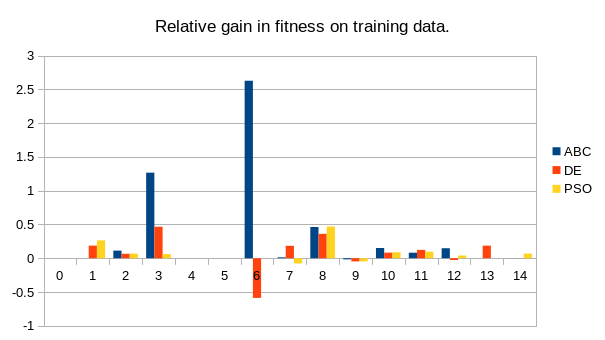
\includegraphics[width=0.5\columnwidth]{figures/hybrid_phases2_mintrainfitness.png}
    \caption{Relative gain in best fitness of training data - 2 phases}
    \end{subfigure}%
    \begin{subfigure}{0.6\textwidth}
    \centering
     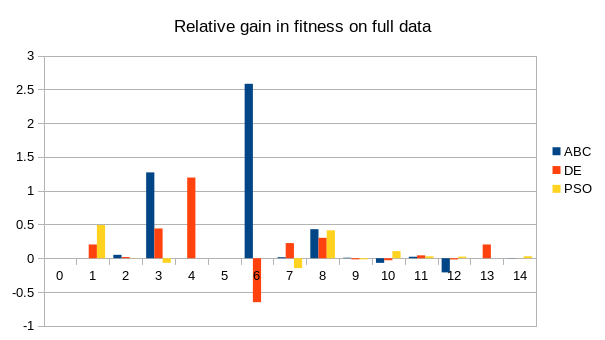
\includegraphics[width=0.5\columnwidth]{figures/hybrid_phases2_minfullfitness.png}
    \caption{Relative gain in best fitness of full data - 2 phases}
    \end{subfigure}
    \begin{subfigure}{0.6\textwidth}
    \centering
    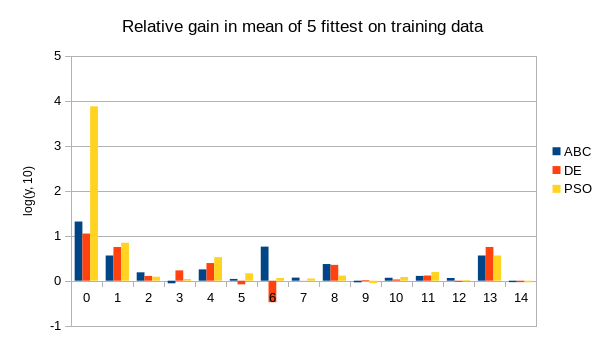
\includegraphics[width=0.5\columnwidth]{figures/hybrid_phases2_meantrainfitness.png}
    \caption{Relative gain in mean fitness of 5 best on training data - 2 phases}
    \end{subfigure}%
    \begin{subfigure}{0.6\textwidth}
    \centering
    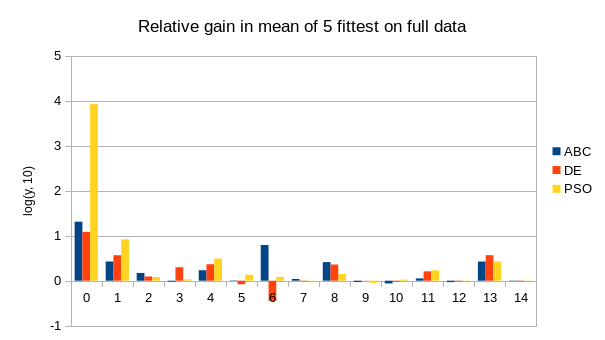
\includegraphics[width=0.5\columnwidth]{figures/hybrid_phases2_meanfullfitness.png}
    \caption{Relative gain in mean fitness of 5 best on full data - 2 phases}
    \label{fig:2phase}
    \end{subfigure}
    \begin{subfigure}{0.6\textwidth}
    \centering
        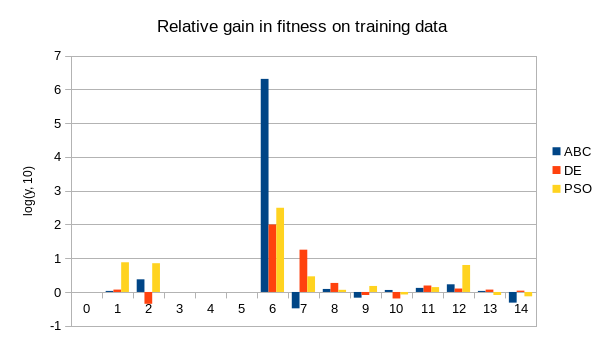
\includegraphics[width=0.5\columnwidth]{figures/hybrid_phases5_mintrainfitness.png}
        \caption{Relative gain in best fitness of training data - 5 phases}
    \end{subfigure}%
    \begin{subfigure}{0.6\textwidth}
    \centering
        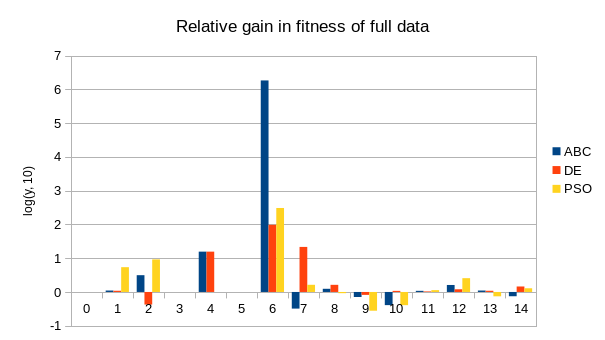
\includegraphics[width=0.5\columnwidth]{figures/hybrid_phases5_minfullfitness.png}
        \caption{Relative gain in best fitness of full data - 5 phases}
    \end{subfigure}
        \begin{subfigure}{0.6\textwidth}
    \centering
        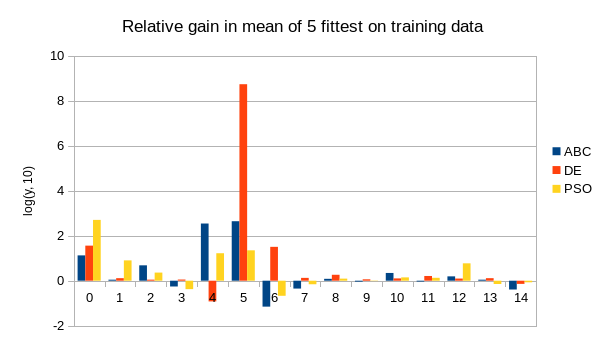
\includegraphics[width=0.5\columnwidth]{figures/hybrid_phases5_meantrainfitness.png}
        \caption{Relative gain in mean fitness of 5 best on training data - 5 phases}
    \end{subfigure}%
    \begin{subfigure}{0.6\textwidth}
    \centering
        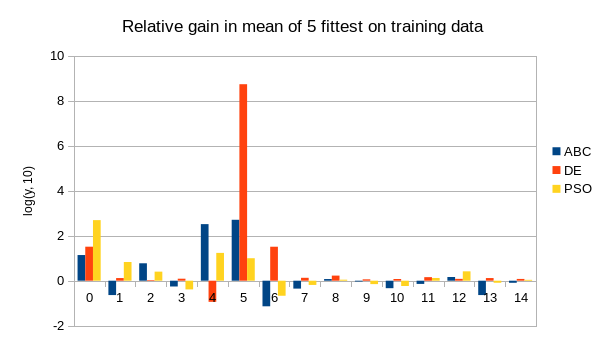
\includegraphics[width=0.5\columnwidth]{figures/hybrid_phases5_meanfullfitness.png}
        \caption{Relative gain in mean fitness of 5 best on full data - 5 phases}
        \label{fig:5phase}
    \end{subfigure}
        \begin{subfigure}{0.6\textwidth}
    \centering
        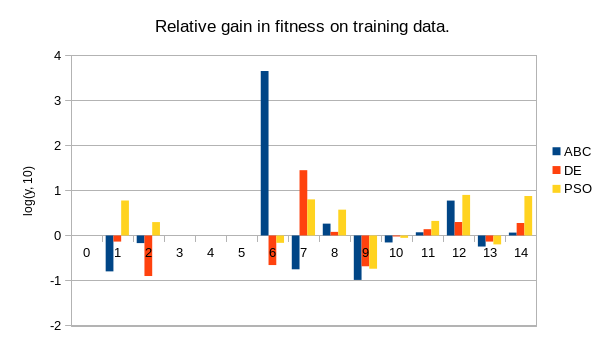
\includegraphics[width=0.5\columnwidth]{figures/hybrid_phases10_mintrainfitness.png}
        \caption{Relative gain in best fitness of training data - 10 phases}
    \end{subfigure}%
    \begin{subfigure}{0.6\textwidth}
    \centering
        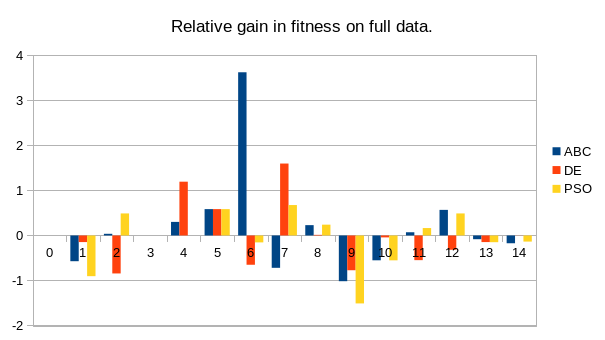
\includegraphics[width=0.5\columnwidth]{figures/hybrid_phases10_minfullfitness.png}
        \caption{Relative gain in best fitness of full data - 10 phases}
    \end{subfigure}
        \begin{subfigure}{0.6\textwidth}
    \centering
        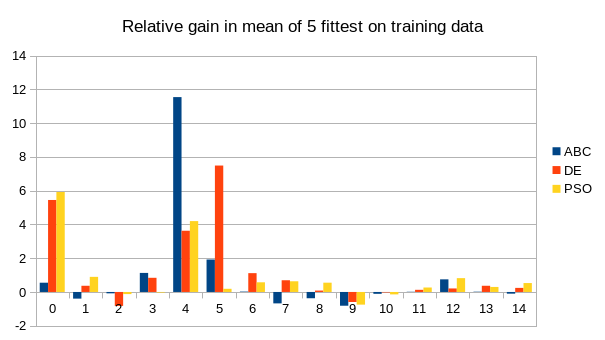
\includegraphics[width=0.5\columnwidth]{figures/hybrid_phases10_meantrainfitness.png}
        \caption{Relative gain in mean fitness of 5 best on training data - 10 phases}
    \end{subfigure}%
    \begin{subfigure}{0.6\textwidth}
    \centering
        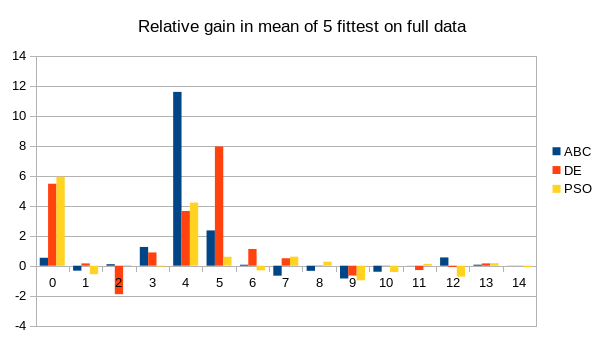
\includegraphics[width=0.5\columnwidth]{figures/hybrid_phases10_meanfullfitness.png}
        \caption{Relative gain in mean fitness of 5 best on full data - 10 phases}
            \label{fig:10phase}
    \end{subfigure}

    \caption{Relative gain of optimizer after 2,5,10 phases.}
%    \label{fig:5phase}
\end{figure*}
\paragraph{10 Phases}
If we observe the convergence after 10 phases we see a more pronounced effect. In Figure \ref{fig:10phase} we see that for several problems the optimizers are no longer improving w.r.t. the unoptimized algorithm. This only holds for the best values. For the mean values the improvements are still significant. It becomes clear that the optimizer can force the algorithm into a local optimum. The correlation between fitness results on the training data and full data is starting to weaken as well, compared to the experiments with 2 and 5 phases. 
Looking at the fitness values for the full data, DE is the more stable algorithm. When it regresses its losses are smaller than the others, while its gains are strongest on the most problems. For the mean fitness of the full data a similar argument can be made, with the exception of problem 2 where DE fails severely.
Another aspect is that after 100 generations the fitness values are extremely small, in the order of 1e-15. We measure the relative gain with respect to the algorithm without an optimizer, but as the fitness values decrease rounding errors start to influence the calculations more and more. The fitness values are approaching the floating point epsilon values. For our implementation epsilon is set at 2.22 e-16. For problem 0, a minimum fitness value of 0 is found after 2 phases. For others far more iterations are needed. We need to make a trade-off in order to be able to compare all 15 problems. Giving each problem an equal budget in iterations is the more fair approach. Another approach is implementing a stop condition that halts within a certain distance of a desired fitness threshold, but this approach is fraught with issues. There is no guarantee exactly how many iterations are needed. This approach requires knowing the problem 'hardness' \cite{GPHardness} in advance, but by the very definition of our problem statement we do not know how hard our problem is. 